
\section{Sensitivity Analysis}

\todo{Introduce, specify what the variables are and present the grahs}

\begin{figure}
        \centering
        \begin{subfigure}[b]{0.5\textwidth}
                \includegraphics[width=\textwidth]{figures/processor_model/ol}
                \label{fig:gull}
        \end{subfigure}%
        \begin{subfigure}[b]{0.5\textwidth}
                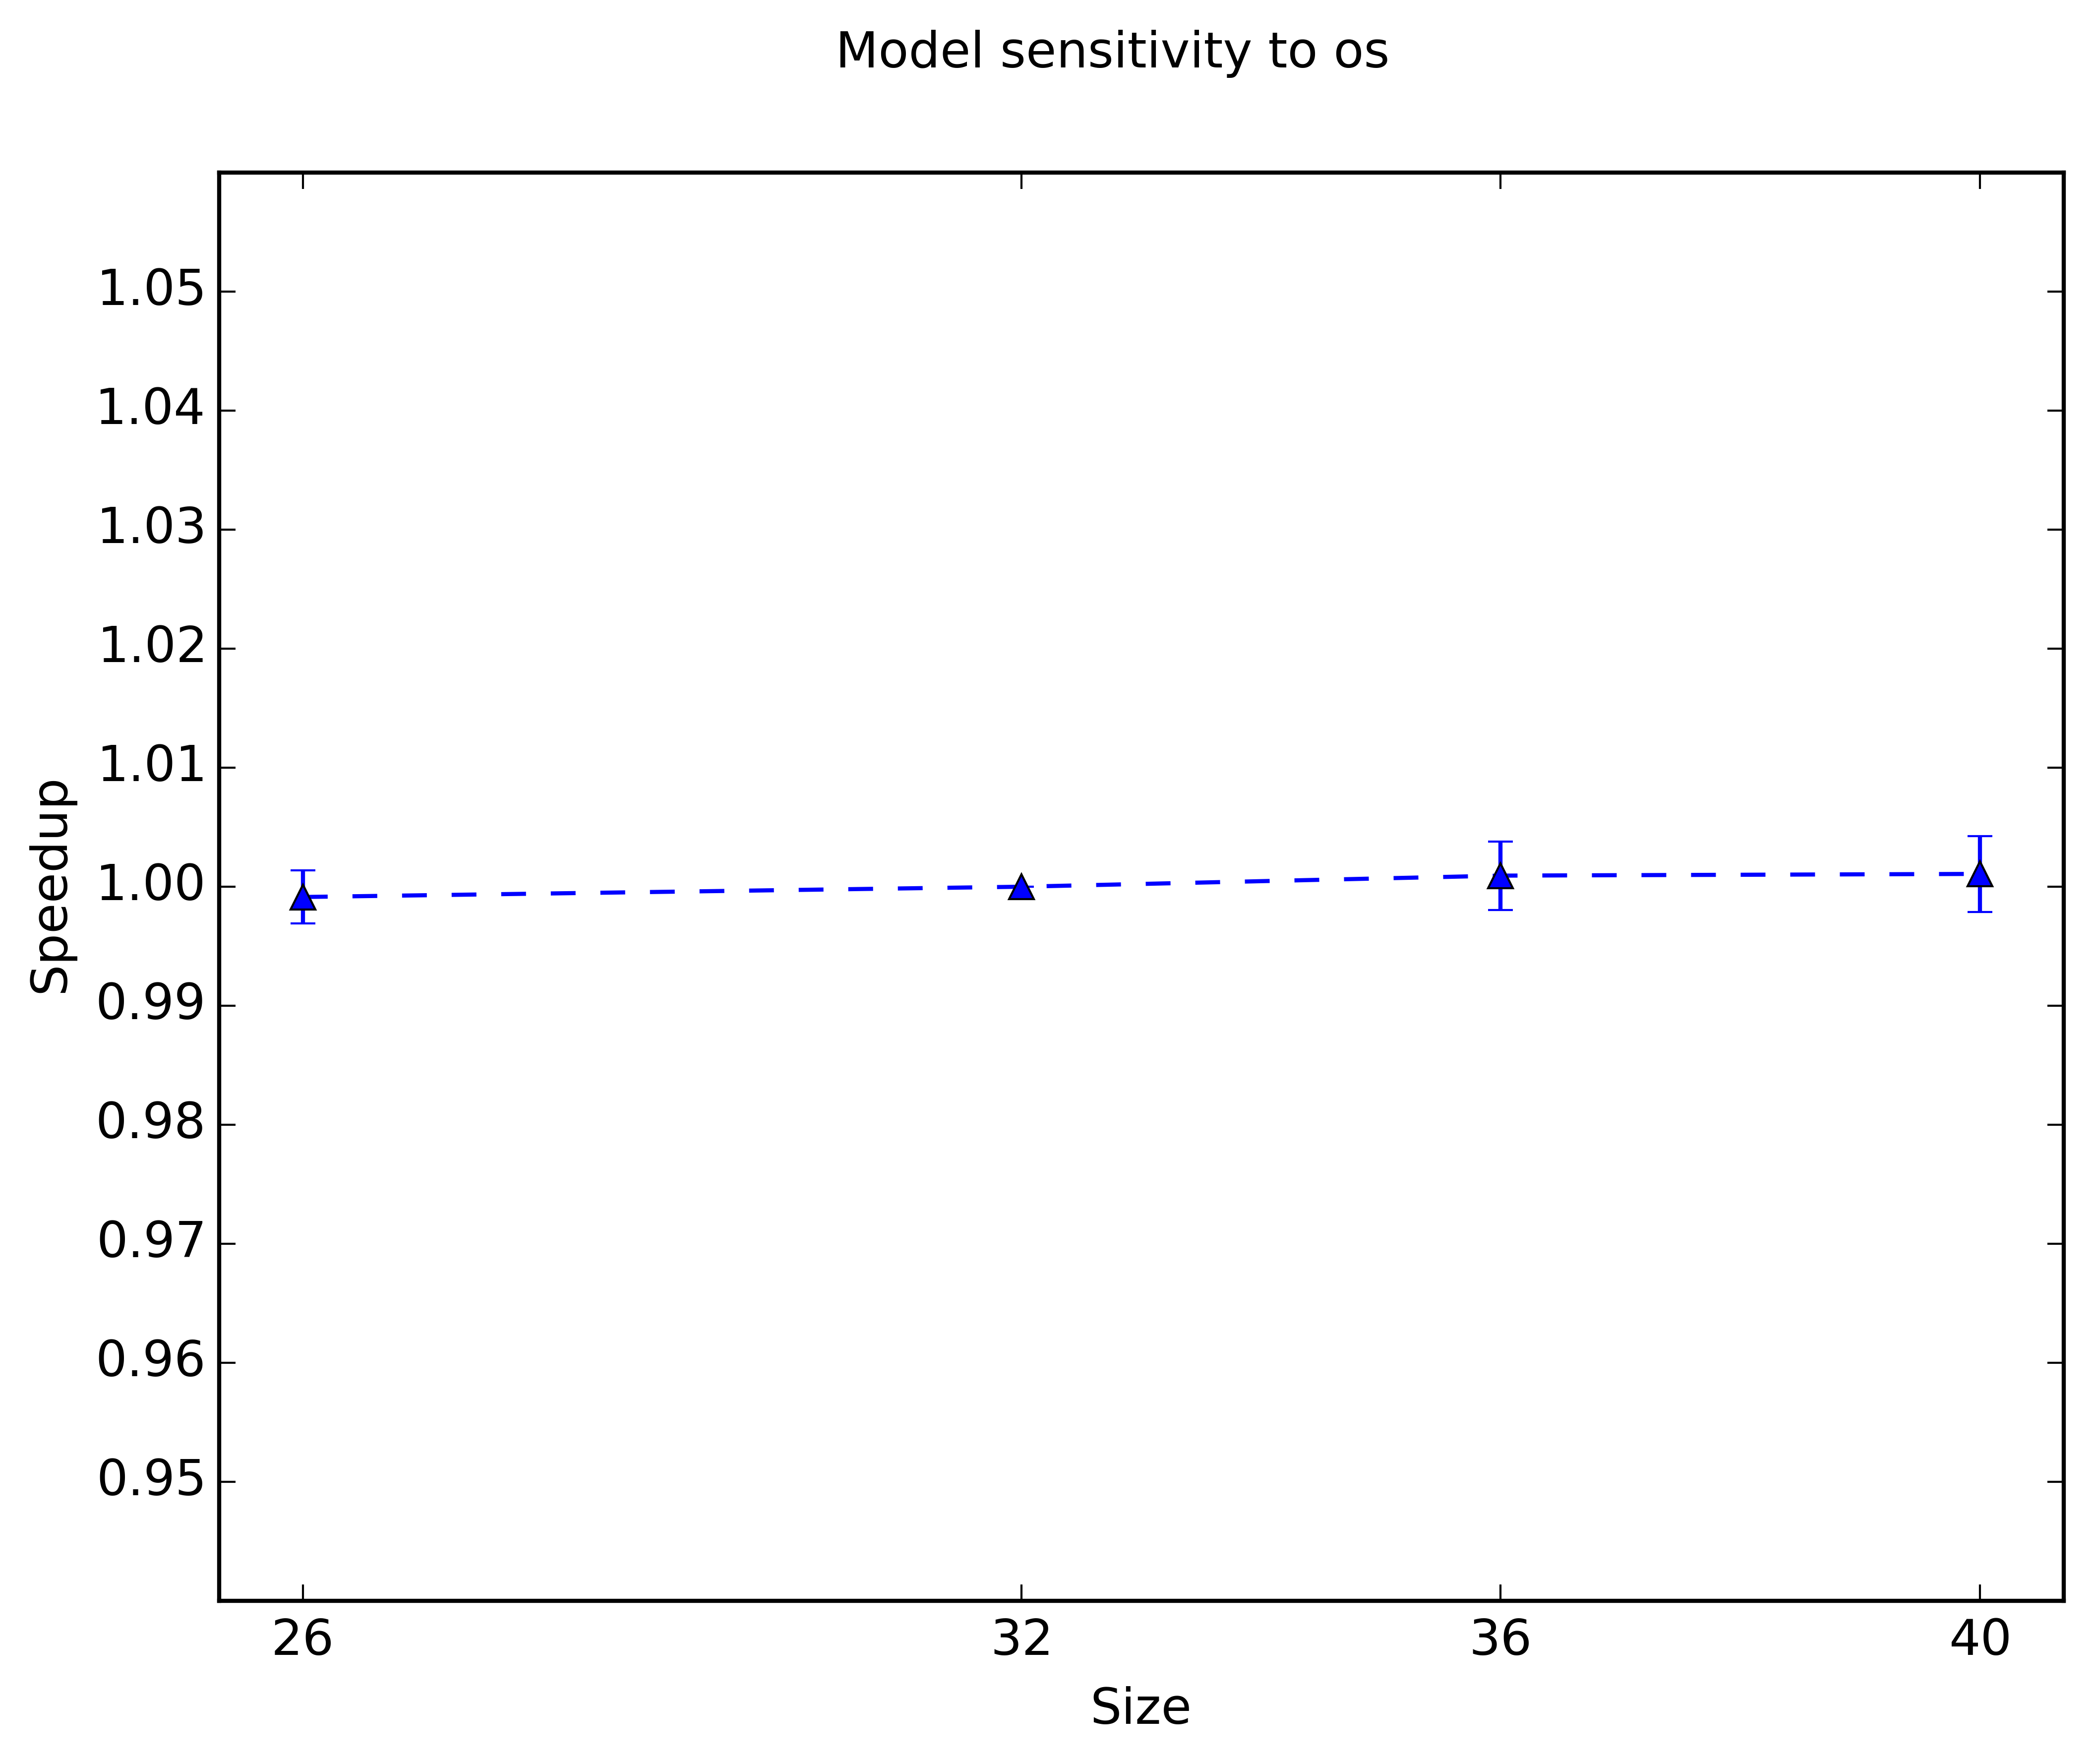
\includegraphics[width=\textwidth]{figures/processor_model/os}
                \label{fig:tiger}
        \end{subfigure}
        \begin{subfigure}[b]{0.5\textwidth}
                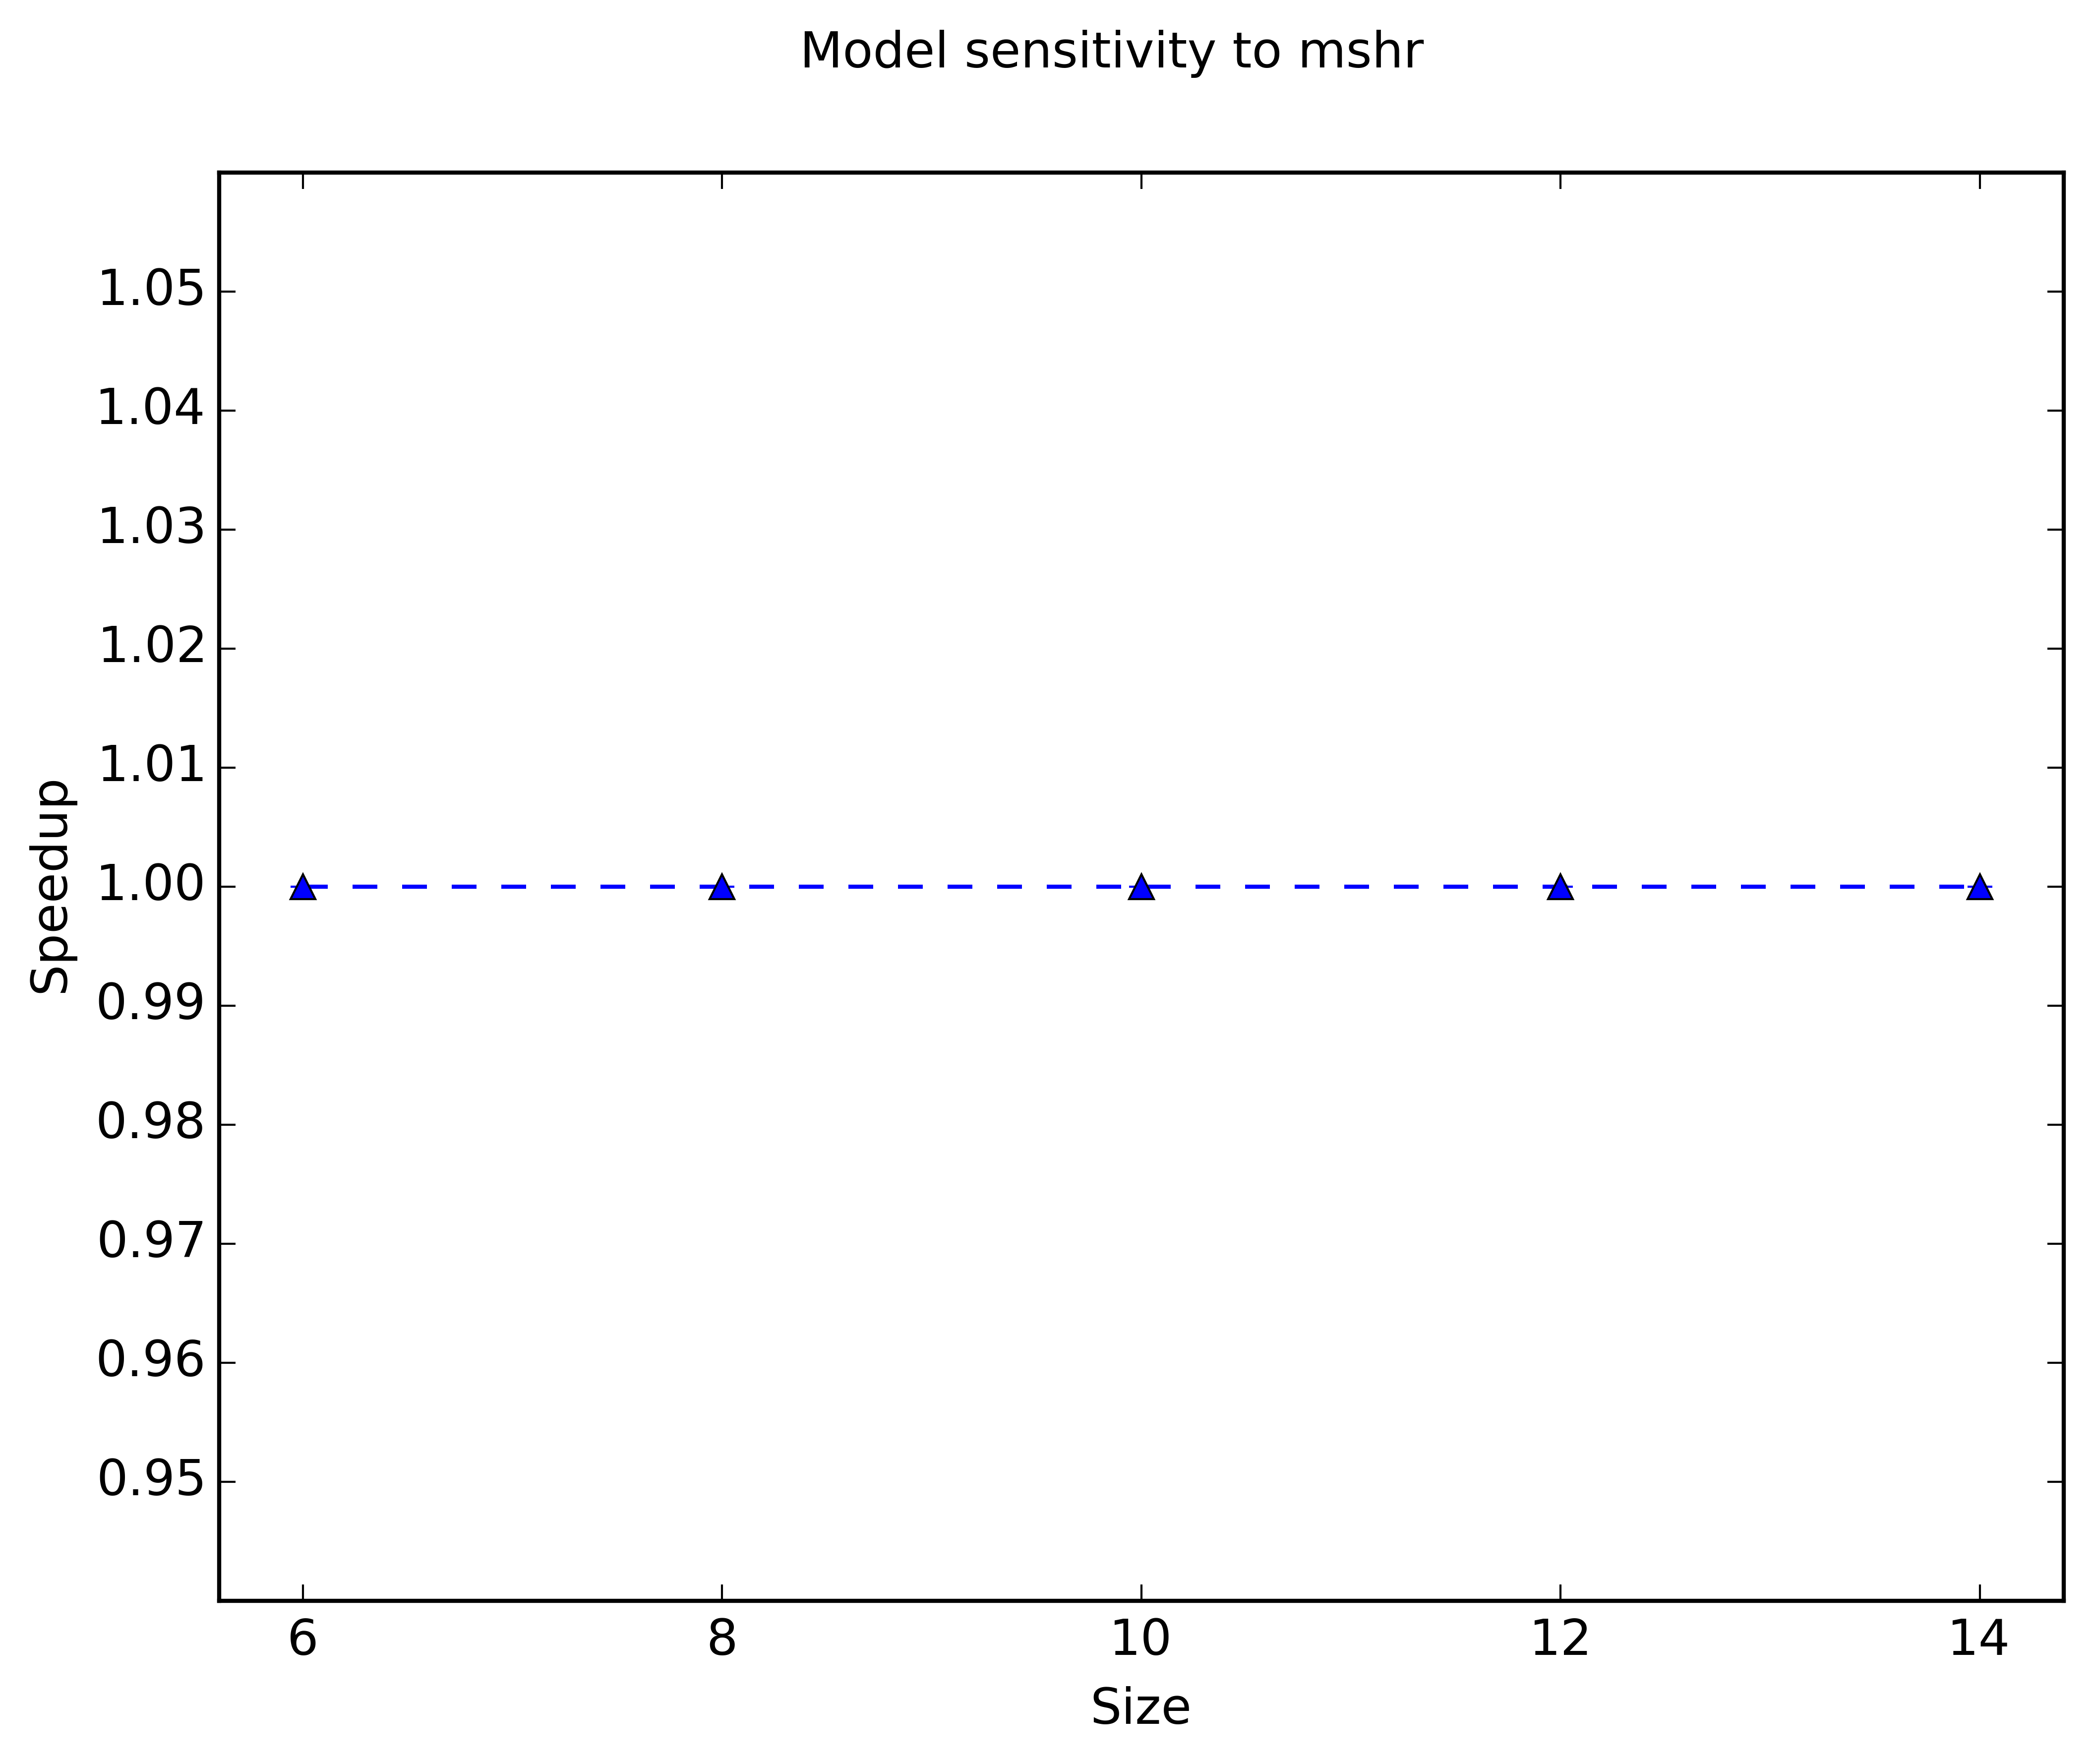
\includegraphics[width=\textwidth]{figures/processor_model/mshr}
                \label{fig:mouse}
        \end{subfigure}%
        \begin{subfigure}[b]{0.5\textwidth}
                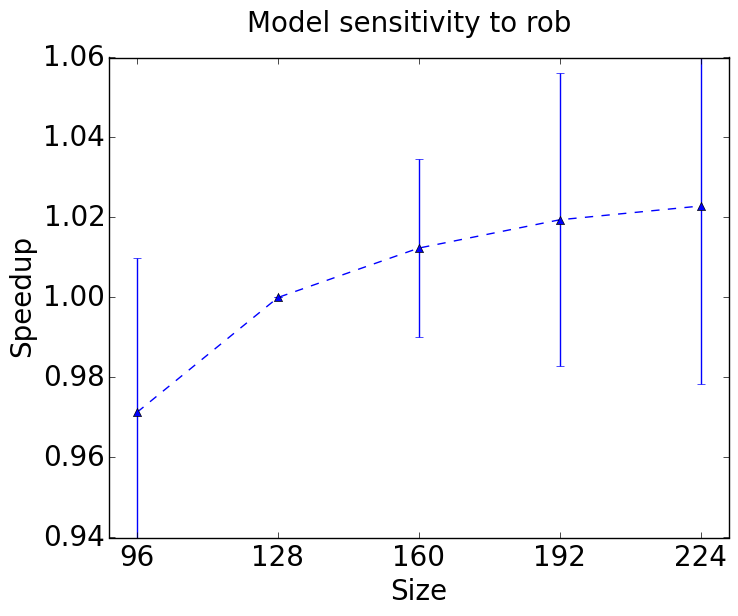
\includegraphics[width=\textwidth]{figures/processor_model/rob}
                \label{fig:mouse}
        \end{subfigure}
        \begin{subfigure}[b]{0.5\textwidth}
                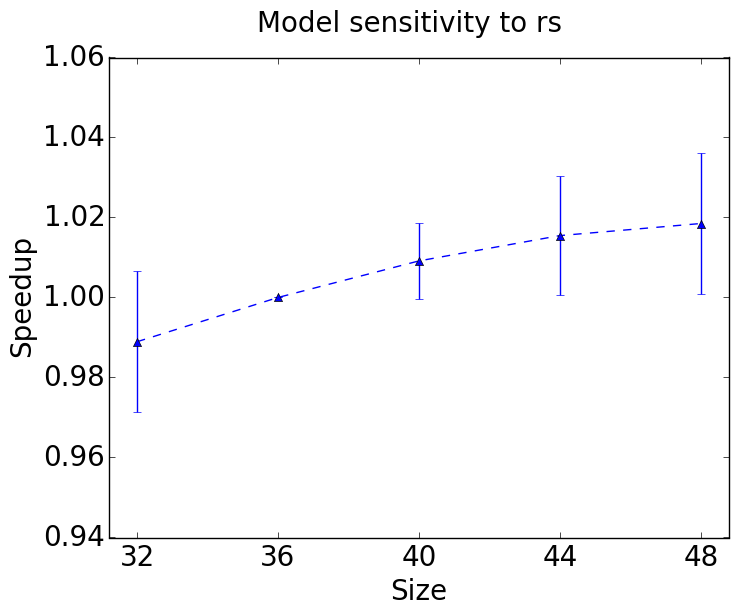
\includegraphics[width=\textwidth]{figures/processor_model/rs}
                \label{fig:mouse}
        \end{subfigure}%
        \caption{Core model property sensitivity}\label{fig:animals}
\end{figure}

No noticable sensitivity to ol, os and mshr changes.

Slight improvement with increasing RS and ROB size, but still less than 3\% with >50\% size increase.
Stddev. outgrows performance gain, we therefor choose to use original model parameters.